\section{eo\-Cellular\-Easy\-EA$<$ EOT $>$ Class Template Reference}
\label{classeo_cellular_easy_e_a}\index{eoCellularEasyEA@{eoCellularEasyEA}}
The abstract cellular easy algorithm.  


{\tt \#include $<$eo\-Cellular\-Easy\-EA.h$>$}

Inheritance diagram for eo\-Cellular\-Easy\-EA$<$ EOT $>$::\begin{figure}[H]
\begin{center}
\leavevmode
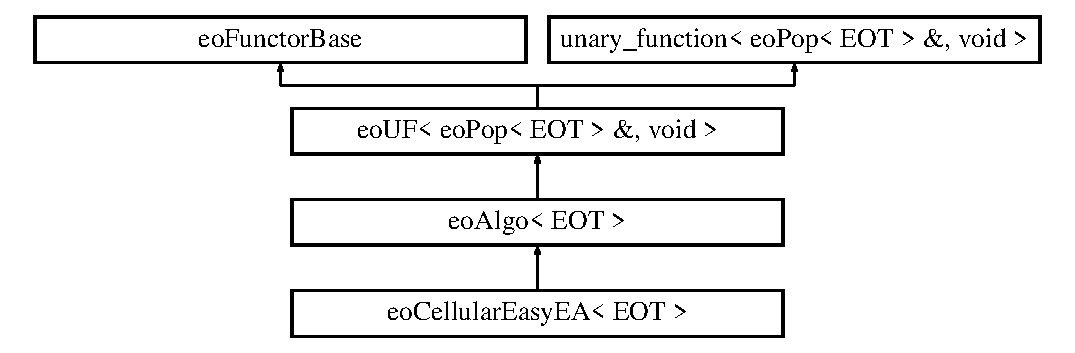
\includegraphics[height=4cm]{classeo_cellular_easy_e_a}
\end{center}
\end{figure}
\subsection*{Public Member Functions}
\begin{CompactItemize}
\item 
{\bf eo\-Cellular\-Easy\-EA} ({\bf eo\-Continue}$<$ {\bf EOT} $>$ \&\_\-cont, {\bf eo\-Eval\-Func}$<$ {\bf EOT} $>$ \&\_\-eval, {\bf eo\-Select\-One}$<$ {\bf EOT} $>$ \&\_\-sel\_\-neigh, {\bf eo\-Bin\-Op}$<$ {\bf EOT} $>$ \&\_\-cross, {\bf eo\-Mon\-Op}$<$ {\bf EOT} $>$ \&\_\-mut, {\bf eo\-Select\-One}$<$ {\bf EOT} $>$ \&\_\-sel\_\-repl)\label{classeo_cellular_easy_e_a_a0}

\begin{CompactList}\small\item\em Two constructors. \item\end{CompactList}\item 
{\bf eo\-Cellular\-Easy\-EA} ({\bf eo\-Continue}$<$ {\bf EOT} $>$ \&\_\-cont, {\bf eo\-Eval\-Func}$<$ {\bf EOT} $>$ \&\_\-eval, {\bf eo\-Select\-One}$<$ {\bf EOT} $>$ \&\_\-sel\_\-neigh, {\bf eo\-Quad\-Op}$<$ {\bf EOT} $>$ \&\_\-cross, {\bf eo\-Mon\-Op}$<$ {\bf EOT} $>$ \&\_\-mut, {\bf eo\-Select\-One}$<$ {\bf EOT} $>$ \&\_\-sel\_\-child, {\bf eo\-Select\-One}$<$ {\bf EOT} $>$ \&\_\-sel\_\-repl)\label{classeo_cellular_easy_e_a_a1}

\item 
void {\bf operator()} ({\bf eo\-Pop}$<$ {\bf EOT} $>$ \&pop)\label{classeo_cellular_easy_e_a_a2}

\begin{CompactList}\small\item\em For a given population. \item\end{CompactList}\end{CompactItemize}
\subsection*{Protected Member Functions}
\begin{CompactItemize}
\item 
virtual {\bf eo\-Pop}$<$ {\bf EOT} $>$ {\bf neighbours} (const {\bf eo\-Pop}$<$ {\bf EOT} $>$ \&pop, int rank)=0\label{classeo_cellular_easy_e_a_b0}

\end{CompactItemize}
\subsection*{Private Attributes}
\begin{CompactItemize}
\item 
{\bf eo\-Continue}$<$ {\bf EOT} $>$ \& {\bf cont}\label{classeo_cellular_easy_e_a_r0}

\item 
{\bf eo\-Eval\-Func}$<$ {\bf EOT} $>$ \& {\bf eval}\label{classeo_cellular_easy_e_a_r1}

\item 
{\bf eo\-Pop\-Loop\-Eval}$<$ {\bf EOT} $>$ {\bf pop\-Eval}\label{classeo_cellular_easy_e_a_r2}

\item 
{\bf eo\-Select\-One}$<$ {\bf EOT} $>$ \& {\bf sel\_\-neigh}\label{classeo_cellular_easy_e_a_r3}

\item 
{\bf eo\-BF}$<$ {\bf EOT} \&, {\bf EOT} \&, bool $>$ \& {\bf cross}\label{classeo_cellular_easy_e_a_r4}

\item 
{\bf eo\-Mon\-Op}$<$ {\bf EOT} $>$ \& {\bf mut}\label{classeo_cellular_easy_e_a_r5}

\item 
{\bf eo\-Select\-One}$<$ {\bf EOT} $>$ \& {\bf sel\_\-child}\label{classeo_cellular_easy_e_a_r6}

\item 
{\bf eo\-Select\-One}$<$ {\bf EOT} $>$ \& {\bf sel\_\-repl}\label{classeo_cellular_easy_e_a_r7}

\end{CompactItemize}


\subsection{Detailed Description}
\subsubsection*{template$<$class EOT$>$ class eo\-Cellular\-Easy\-EA$<$ EOT $>$}

The abstract cellular easy algorithm. 



Definition at line 38 of file eo\-Cellular\-Easy\-EA.h.

The documentation for this class was generated from the following file:\begin{CompactItemize}
\item 
eo\-Cellular\-Easy\-EA.h\end{CompactItemize}
